\documentclass[11pt, oneside]{article} 
\usepackage{geometry}
\geometry{letterpaper} 
\usepackage{graphicx}
	
\usepackage{amssymb}
\usepackage{amsmath}
\usepackage{parskip}
\usepackage{color}
\usepackage{hyperref}

\graphicspath{{/Users/telliott_admin/Tex/png/}}
% \begin{center} 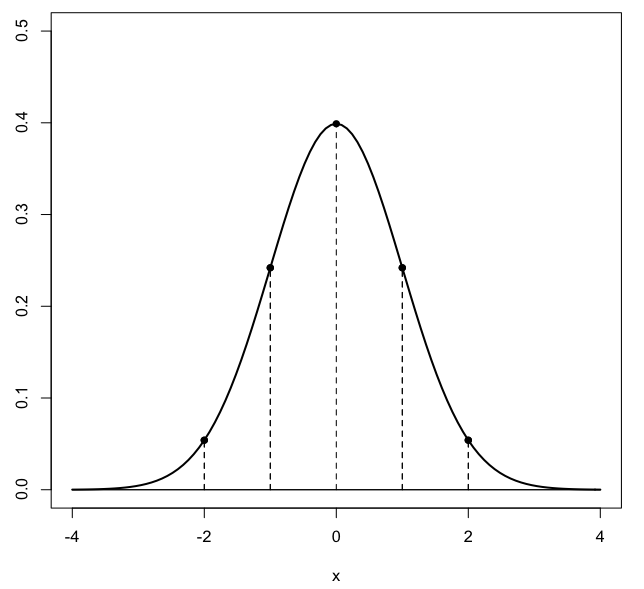
\includegraphics [scale=0.4] {gauss3.png} \end{center}

\title{Powers of sine and cosine}
\date{}

\begin{document}
\maketitle
\Large

Occasionally, we run into higher powers of the sine and or the cosine.

This chapter explains how to figure these out using integration by parts, but it is complicated enough that if you can, it is probably better to look up the answer in a table of integrals.

If the integrand contains only integral powers like $\sin^m x$ and $\cos^n x$, then there are two cases.  If both $m$ and $n$ are even (or only one is present and that power is even), you can use the formula we will develop here.  Otherwise, simply separate out one factor of $\sin x$ or $\cos x$ to combine with $dx$, like this:

\[ \int \sin^5 x \cos^4 x \ dx \]
\[ = \int \sin^4 x \cos^4 x \sin x \ dx \]
\[ = \int (1- \cos^2 x)^2 \cos^4 x \sin x \ dx \]
\[ = \int (\cos^4 x - 2 \cos^6 x + \cos^8 x) \sin x \ dx \]
This is just
\[ -\int u^4 - 2u^6 + u^8 \ du \]

To handle the case with $m$ and $n$ both even, first use the identity $\sin^2 + \cos^2 = 1$ to convert to all sine or all cosine.  Converting the function with the smaller exponent will give the least complicated expression.  Now we have an integral of only sine or only cosine raised to an even power.  We will use $n$ to represent that power.  Let's do cosine first:
\[ \int \cos^n x \ dx \]
We use integration by parts:
\[ u = \cos^{n-1} x \]
\[ du = -(n-1)\cos^{n-2} x \sin x \ dx \]
\[ dv = \cos x \ dx \]
\[ v = \sin x \]

So $\int \cos^n x \ dx$ is $\int u \ dv$ and this is equal to $uv - \int v \ du$.  We have (reversing terms and writing $vu$):
\[ \sin x \cos^{n-1} x + \int \sin x (n-1) \cos^{n-2} x \sin x \ dx \]

The last term is
\[ \sin x (n-1) \cos^{n-2} x \sin x \]
\[ = (n-1) \cos^{n-2} x \sin^2 x  \]
\[ = (n-1) \cos^{n-2} x \ (1 - \cos^2 x)  \]
\[ = (n-1) \cos^{n-2} x - (n-1) \cos^n x \]
The trick is that although we have produced $- (n-1) \cos^n x$ on the right-hand side, this can be moved to the left-hand side, and added to the expression we started with.  Placing the above result under the integral and moving all of the $\cos^n x$ terms to the left-hand side, we obtain
\[ n \int \cos^n x \ dx =   \sin x \cos^{n-1} x +  (n-1) \int \cos^{n-2} x \ dx \]

We divide by $n$ to obtain the general formula.  
\[ \boxed{\int \cos^n x \ dx =   \frac{1}{n} \sin x \cos^{n-1} x +  \frac{n-1}{n} \int \cos^{n-2} x \ dx} \]

A few specific examples:
\[ \int \cos^2 x \ dx =   \frac{1}{2} \sin x \cos x +  \frac{1}{2} \int \cos^{0} x \ dx \]
\[ = \frac{1}{2}(\sin x \cos x + x)  \]
\[ \int \cos^4 x \ dx =   \frac{1}{4} \sin x \cos^3 x +  \frac{3}{4} \int \cos^{2} x \ dx \]
\[ = \frac{1}{4} \sin x \cos^3 x +  \frac{3}{8} (\sin x \cos x + x)  \]
\[ \int \cos^6 x \ dx =   \frac{1}{6} \sin x \cos^5 x +  \frac{5}{6} \int \cos^{4} x \ dx \]
\[ = \frac{1}{6} \sin x \cos^5 x +  \frac{5}{24} \sin x \cos^3 x +  \frac{5}{16} (\sin x \cos x + x)  \]

We will work out the formula for sine below, but notice:
\[ \sin^2 x + \cos^2 x = 1 \]
\[ \int \sin^2 x \ dx + \int \cos^2 x \ dx = \int dx = x \]
Looking at the formula for cosine squared
\[ \int \cos^2 x \ dx = \frac{1}{2}(\sin x \cos x + x)  \]
it should be clear that we will end up with the same formula for sine squared, but just flip the sign on the term $\sin x \cos x$ to make it go away in the sum.  Let's see:
\[ \int \sin^n x \ dx \]

We use integration by parts:
\[ u = \sin^{n-1} x \]
\[ du = (n-1)\sin^{n-2} x \cos x \ dx \]
\[ dv = \sin x \ dx \]
\[ v = -\cos x \]
For $uv - \int v \ du$ we have:
\[ \sin^{n-1} x (- \cos x) - \int (- \cos x) (n-1)\sin^{n-2} x \cos x \ dx \]

Just as before, the last term is
\[ \sin^{n-2} x \cos^2 x \]
\[ = \sin^{n-2} x (1 - \sin^2 x) \]
\[ = \sin^{n-2} x - \sin^n x \]
So the whole thing is:
\[ \int \sin^n x \ dx = -\sin^{n-1} x \cos x + (n-1) \int \sin^{n-2} x \ dx - (n-1) \int \sin^4 x \ dx \]
\[ n \int \sin^n x \ dx = -\sin^{n-1} x \cos x + (n-1) \int \sin^{n-2} x \ dx  \]
\[ \boxed{\int \sin^n x \ dx = - \frac{1}{n} \sin^{n-1} x \cos x + \frac{n-1}{n} \int \sin^{n-2} x \ dx}  \]

So for $\sin^2 x$:
\[ \int \sin^2 x \ dx = - \frac{1}{2} \sin^{n-1} x \cos x + \frac{1}{2} \int \ dx  \]
\[ \int \sin^2 x \ dx = \frac{1}{2} (- \sin^{n-1} x \cos x + x)  \]
As predicted, we have simply switched the sign on the first term.


\end{document}